\begin{figure}

\begin{minipage}{\linewidth}
\begin{subfigure}[b]{0.692\linewidth}
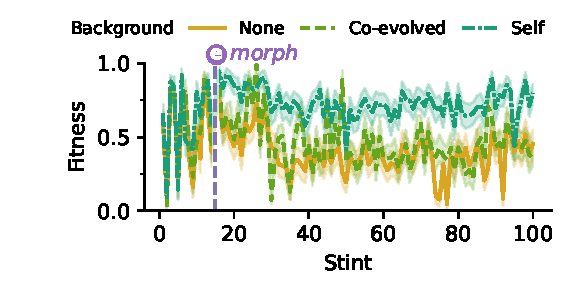
\includegraphics[width=\linewidth, trim=0.8cm 0 0 0, clip]{binder-2025-11-30-external-selfbb-truebb.ipynb/binder/teeplots/2025-11-30-external-selfbb-truebb/hue=kind1+style=kind1+viz=lineplot+x=competition-stint+y=focal-prevalence+ext=.pdf}
\footnotesize
\vspace{-4.25ex}
\caption{stints 0 to 100}
\label{fig:fitness-background:timeseries}
\end{subfigure}%
\begin{subfigure}[b]{0.308\linewidth}
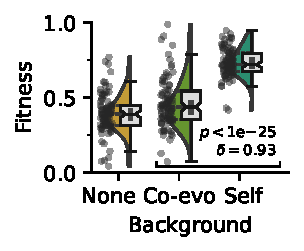
\includegraphics[width=\linewidth, trim=1.3cm 0 0 0.1cm, clip]{binder-2025-11-30-external-selfbb-truebb.ipynb/binder/teeplots/2025-11-30-external-selfbb-truebb/hue=kind+inner=quartile+viz=violinplot+x=kind+y=focal-prevalence+ext=.pdf}
\footnotesize
\vspace{-4.25ex}
\caption{stints 15 to 100}
\label{fig:fitness-background:distribution}
\end{subfigure}
\end{minipage}

\caption{%
\textbf{Patterned growth creates biogenic niche.}
\footnotesize
Around stint 15, fitness of case study strain in self-context diverges significantly above other contexts.
``None'' background competitions are initialized 50\%/50\% between compared strains; otherwise, competitions are initialized 25\%/25\%/50\% between compared strains and background.
Shaded bands are bootstrap 95\% CI.
Mann-Whitney test reported.
}
\label{fig:fitness-background}
\end{figure}
